%Copyright 2014 Jean-Philippe Eisenbarth
%This program is free software: you can 
%redistribute it and/or modify it under the terms of the GNU General Public 
%License as published by the Free Software Foundation, either version 3 of the 
%License, or (at your option) any later version.
%This program is distributed in the hope that it will be useful,but WITHOUT ANY 
%WARRANTY; without even the implied warranty of MERCHANTABILITY or FITNESS FOR A 
%PARTICULAR PURPOSE. See the GNU General Public License for more details.
%You should have received a copy of the GNU General Public License along with 
%this program.  If not, see <http://www.gnu.org/licenses/>.

%Based on the code of Yiannis Lazarides
%http://tex.stackexchange.com/questions/42602/software-requirements-specification-with-latex
%http://tex.stackexchange.com/users/963/yiannis-lazarides
%Also based on the template of Karl E. Wiegers
%http://www.se.rit.edu/~emad/teaching/slides/srs_template_sep14.pdf
%http://karlwiegers.com
\documentclass{scrreprt}
\usepackage{listings}
\usepackage{graphicx}
\usepackage{underscore}
\usepackage[bookmarks=true]{hyperref}
\usepackage[utf8]{inputenc}
\usepackage[english]{babel}
\usepackage[section]{placeins}
\hypersetup{
    bookmarks=false,    % show bookmarks bar?
    pdftitle={Software Requirement Specification},    % title
    pdfauthor={Jean-Philippe Eisenbarth},                     % author
    pdfsubject={TeX and LaTeX},                        % subject of the document
    pdfkeywords={TeX, LaTeX, graphics, images}, % list of keywords
    colorlinks=true,       % false: boxed links; true: colored links
    linkcolor=blue,       % color of internal links
    citecolor=black,       % color of links to bibliography
    filecolor=black,        % color of file links
    urlcolor=blue,        % color of external links
    linktoc=page            % only page is linked
}%
\def\myversion{1.0 }
\date{}
%\title
\usepackage{hyperref}
\begin{document}

\begin{flushright}
    \rule{16cm}{5pt}\vskip1cm
    \begin{bfseries}
        \Huge{SOFTWARE ANALYSIS\\ AND DESIGN}\\
        \vspace{1.9cm}
        for\\
        \vspace{1.9cm}
        Book Shop Automation Software\\
        \vspace{1.9cm}
        \LARGE{Version \myversion approved}\\
        \vspace{1.8cm}
        Presented by\\
        \vspace{0.5cm}
        Rameshwar Bhaskaran \textbf{(14CS30027)} \\
        Aditya Bhagwat \textbf{(14CS30002)} \\
        Group 55\\
        \vspace{1.3cm}
        IIT Kharagpur\\    
       
        \today\\
    \end{bfseries}
\end{flushright}

\tableofcontents

%\chapter*{Revision History}

%\begin{center}
 %   \begin{tabular}{|c|c|c|c|}
  %      \hline
	%    Name & Date & Reason For Changes & Version\\
     %   \hline
	  %  21 & 22 & 23 & 24\\
       % \hline
	   % 31 & 32 & 33 & 34\\
       % \hline
    %\end{tabular}
%\end{center}
\chapter{Introduction}
\section{Purpose}
The purpose of this document is to document the detailed design specifications of the BAS. It contains analysis and dissection of the requirements with the help of diagrams.

\section{Analysis of stakeholders}
\subsection{Customer}
The main focus of this software is to satisfy customer's user experience in finding their book of choice. The customer is given least number of priveleges as he cannot control the database.

\subsection{Employee}
The employee is a generalised form of any person associated with the shop who has read/write permissions on the database. There can be multiple employees in the shop. The employee can update the inventory when new stock has arrived or when books are defective/sold.

\subsection{Sales Clerk}
The sales clerk is the employee who directly handles transactions with the customer. His main job is to receive the book's details(ISBN code) and appropriately generate the receipt, apart from the normal employee's priveleges.

\subsection{Manager}
The manager controls the requests and decides whether a particular book has to be procured from a vendor ,depending on the demand for the book, apart from the normal tasks a sales clerk can do.

\subsection{Owner}
The owner of the book shop is given the highest privelege. Apart from the tasks a manager can do, the owner can view books which have fallen below the threshold level and order them. There is only one owner in the shop.
 
\section{Relevant Study} 

A number of related softwares were studied and one common feature which was found to enhance user experience multifold was the use of a "cart" wherein the user can add items to it. This prevents a highly impractical situation where the user has to bill one book at a time.

\section{Alternatives to used tools}

The software is built with the Java as the main language and is designed to work on Linux and Windows. Linux will be the most preferred platform however. Swing is used for building the GUI and the database vendor used is MySQL. JavaFX is also a good alternative as it has good animations and transitions. Also the PDF generation library used is iText library. The alternatives were considered also: \\ \\
\textbf{Swing}
\begin{itemize}
\item JavaFX 
\end{itemize} 
\textbf{MySQL}
\begin{itemize}
\item ODBMS 
\item ORDBMS
\end{itemize}



\textbf{iText}
\begin{itemize}
\item PdfBox
\item PdfClown
\end{itemize} 



\section{Criteria to evaluate alternatives}
\begin{itemize}
\item 
 Swing provides a stable user interface and is the industry's standard.Further, the support and documentation are in Swing's favour. JavaFX has a sleek interface and better looks , hence the software can also 
 be built in JavaFX to improve user interface look.
\item MySQL was preferred over ORDBMS and ODBMS because of its superior user community and popularity.
\item iText library is the most popular Pdf generation library. As it had a richer number of features and a superior community,this was chosen
\end{itemize}


\section{Unusual circumstances}
As is the case with any software, the user session will be destroyed if the software is closed unexpectedly, like in the case of power shutdown etc. However the database is not lost as it is a persistent data. User session loss wouldn't affect the software much as no valuable data would be lost.

% SA SD DOCUMENT starts here
\clearpage

\chapter{UML Diagrams}
\section{Use Case Diagrams}
\begin{figure}[!htb]
  \includegraphics[width=\linewidth]{"/home/rameshwar/FinalAssignmnet/BAS/SA-SD/images/Use Case Diagrams/Customer".jpg}
  \caption{Customer related use cases.}
  \label{fig:usecase}
\end{figure}

\begin{figure}[!htb]
  \includegraphics[width=\linewidth]{"/home/rameshwar/FinalAssignmnet/BAS/SA-SD/images/Use Case Diagrams/General Employee".jpg}
  \caption{Employee related use cases.}
  \label{fig:usecase1}
\end{figure}


\section{Class Diagram}
\begin{figure}[!htb]
  \includegraphics[width=\linewidth]{"/home/rameshwar/FinalAssignmnet/BAS/SA-SD/images/Class Diagrams/cdFinal".jpg}
  \caption{Class Diagram.}
  \label{fig:classdiagram}
\end{figure}
\clearpage
\section{Sequence Diagrams}
\subsection{Book query and transactions}
\begin{figure}[!htb]
  \includegraphics{"/home/rameshwar/FinalAssignmnet/BAS/SA-SD/images/Sequence Diagrams/Book query and transactions".jpg}
  \caption{Book related transactions.}
  \label{fig:seqdiagram}
\end{figure}
\clearpage

\subsection{Generate receipt}
\begin{figure}[!htb]
  \includegraphics{"/home/rameshwar/FinalAssignmnet/BAS/SA-SD/images/2".jpg}
  \caption{Sequence for generating receipt.}
  \label{fig:seqdiagram}
\end{figure}


\subsection{Procurement of books}
\begin{figure}[!htb]
  \includegraphics{"/home/rameshwar/FinalAssignmnet/BAS/SA-SD/images/Sequence Diagrams/ProcureBooks".jpg}
  \caption{Sequence for procuring the book.}
  \label{fig:seqdiagram}
\end{figure}

\clearpage

\subsection{Update inventory}
\begin{figure}[!htb]
  \includegraphics{"/home/rameshwar/FinalAssignmnet/BAS/SA-SD/images/Sequence Diagrams/UpdateInventory".jpg}
  \caption{Sequence for updating the inventory.}
  \label{fig:seqdiagram}
\end{figure}

\subsection{View requests}
\begin{figure}[!htb]
  \includegraphics{"/home/rameshwar/FinalAssignmnet/BAS/SA-SD/images/Sequence Diagrams/View requests".jpg}
  \caption{Sequence for viewing requests.}
  \label{fig:seqdiagram}
\end{figure}

\clearpage
\section{Communication Diagrams}
\subsection{Book query and transactions}
\begin{figure}[!htb]
  \includegraphics[width=\linewidth]{"/home/rameshwar/FinalAssignmnet/BAS/SA-SD/images/Communication Diagrams/Book query and transactions1".jpg}
   \label{fig:seqdiagram}
\end{figure}

\subsection{Generate receipt}
\begin{figure}[!htb]
  \includegraphics[width=\linewidth]{"/home/rameshwar/FinalAssignmnet/BAS/SA-SD/images/1".jpg}

  \label{fig:seqdiagram}
\end{figure}

\clearpage
\subsection{Procure books}
\begin{figure}[!htb]
  \includegraphics[width=\linewidth]
  {"/home/rameshwar/FinalAssignmnet/BAS/SA-SD/images/Communication Diagrams/ProcureBooks".jpg}
   \label{fig:seqdiagram}
\end{figure}


\subsection{Update inventory}
\begin{figure}[!htb]
  \includegraphics[width=\linewidth]
  {"/home/rameshwar/FinalAssignmnet/BAS/SA-SD/images/Communication Diagrams/UpdateInventory".jpg}
   \label{fig:seqdiagram}
\end{figure}


\subsection{View requests}
\begin{figure}[!htb]
  \includegraphics[width=\linewidth]
  {"/home/rameshwar/FinalAssignmnet/BAS/SA-SD/images/Communication Diagrams/View requests".jpg}
   \label{fig:seqdiagram}
\end{figure}

\section{Activity Diagrams}

\subsection{Manager's activity}
\begin{figure}[!htb]
  \includegraphics[width=\linewidth]
  {"/home/rameshwar/FinalAssignmnet/BAS/SA-SD/images/Activity Diagrams/Manager".jpg}
   \label{fig:seqdiagram}
\end{figure}

\subsection{Book query}
\begin{figure}[!htb]
  \includegraphics[width=\linewidth]
  {"/home/rameshwar/FinalAssignmnet/BAS/SA-SD/images/Activity Diagrams/Query for book".jpg}
   \label{fig:seqdiagram}
\end{figure}
\clearpage
\subsection{Stock arrival}
\begin{figure}[!htb]
  \includegraphics[width=\linewidth]
  {"/home/rameshwar/FinalAssignmnet/BAS/SA-SD/images/Activity Diagrams/Stock arrival".jpg}
   \label{fig:seqdiagram}
\end{figure}
\clearpage
\section{State diagrams}
\subsection{Book}
\begin{figure}[!htb]
  \includegraphics[width=\linewidth]
  {"/home/rameshwar/FinalAssignmnet/BAS/SA-SD/images/State Diagrams/Book".jpg}
   \label{fig:statediagram}
\end{figure}

\clearpage
\subsection{Cart}
\begin{figure}[!htb]
  \includegraphics[width=\linewidth]
  {"/home/rameshwar/FinalAssignmnet/BAS/SA-SD/images/State Diagrams/Cart".jpg}
   \label{fig:statediagram}
\end{figure}
\clearpage
\subsection{Order}
\begin{figure}[!htb]
  \includegraphics
  {"/home/rameshwar/FinalAssignmnet/BAS/SA-SD/images/State Diagrams/Order".jpg}
   \label{fig:statediagram}
\end{figure}

\chapter{System analysis}

\section{System Parameters}
The software is built in Java and using Swing library for GUI. The database used is MySQL and JPA/Hibernate framework is used for ORM mapping. The main external library used is the iText library for generating the sales receipt in pdf format and  as mentioned before.
The external hardware necessary is the printer to enable printing of the sales receipt. The software does not need networking in this version of the software as a local database is used. 

\section{Software Analysis}

\subsection{Level 0}

The design flow of the diagram is shown below.

\begin{figure}
\includegraphics[width=\linewidth]{"/home/rameshwar/FinalAssignmnet/BAS/SA-SD/CDfinal".png}
\caption{Context Diagram}
\end{figure}

It provides the functionality of the application and shows interactions between the main players and the BAS.
The main parts of the system are :

\begin{itemize}
\item \textbf{BAS :} \\
This is the software which handles books in the shop. It has many features like query book, viewing statistics etc.

\item \textbf{Employee :}\\
He/she is the basic employee of the shop. He can update the inventory whenever needed.

\item \textbf{Customer :} \\
This stakeholder is the main person who the software caters for. However the least privilege is also given to the same.

\item \textbf{Sales Clerk :}\\
The sales clerk is a superior employee who handles transactions directly with the customer. He is in-charge of generating appropriate receipt and handle monetary transactions.

\item \textbf{Manager :} \\
The manager is a main employee who is in-charge of the functioning of the shop. He is as powerful as the owner when it comes to normal shop adminstration. However ,as expected the owner has obviously more privileges than the employee.

\item \textbf{Owner} \\
The owner of the shop is given the highest privileges.He can do all that a manager can do , and also view books which have fallen below a threshold value and procure them when required. \\

All operations are time efficient as the database operations are already optimised by the database vendor(MySQL).
\end{itemize}
\clearpage
\subsection{Level 1}
As is the case of software analysis , Level 1 gives an in-depth view of the software and intends to give a thorough analysis of the same. The above shows the dataflow diagram. 


\begin{figure}
\includegraphics[width=\linewidth]{"/home/rameshwar/FinalAssignmnet/BAS/SA-SD/Data Flow Diagramfinalest".png}
\caption{Data flow diagram}
\end{figure}


\section{Database Design}
The software needs to store the following details:
\begin{itemize}
\item Books
\item Employee details
\item Login details
\item Sales invoices/details for the day
\item Increment Requests
\item Requests for new books
\end{itemize}

The database design will have to include each point as a table. A foreign key can be used between the Employee table and Login details table. \\

\section{Structural analysis}
The above diagram describes the basic structural flow of the BAS. 
\begin{figure}
\includegraphics[width=\linewidth]{"/home/rameshwar/FinalAssignmnet/BAS/SA-SD/StructuralAnalysis".jpg}
\end{figure}

\section{Global system architecture}
The software is built using Object Oriented Programming concepts and the Model-View-Controller model is used for working and organisation of classes. 
\subsection{Class Organisation}
As depicted in the class diagram, the classes have been organised to model the real-life situation, as is the philosophy of OOP. \\ 
The \textbf{Book} class is the class that stores Book attributes. The employee relations are modelled by the below diagram

\begin{figure}
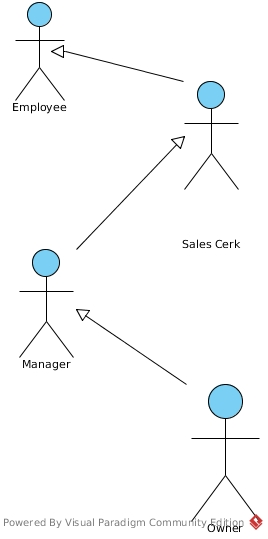
\includegraphics{Actors.jpg}
\caption{The relationship between employees}
\end{figure} 

\clearpage
The \textbf{employee} related classes have 
\begin{itemize}
\item \textbf{Employee}
\item \textbf{Sales Clerk}
\item \textbf{Manager}
\item \textbf{Owner}
\end{itemize} 

The software doesn't however need customer details as it is a small book shop and the process of collecting customer details may hinder user experience. However to implement a mailing system, we require the customer's email address and other minor details for notification. \\

The \textbf{requests} field have two types and uses three classes :
\begin{itemize}
\item \textbf{RequestOrder} \emph{(abstract)}
\item \textbf{NotInStock} 
\item \textbf{NotInCollection}
\end{itemize} 

\section{Other features/implementations}
To give a good recommendation system and to correct spelling mistakes, the edit distance algorithm is employed. Also, to give proper queries, string matching algorithms are used to improve the recommendation engine.

\section{Coding style}
The following style is used for the coding this software.
\begin{itemize}
\item Class names begin with a capital letter
\item Function names start with a small letter and then follow camel case in case of multiple words \emph{i.e} \textbf{\emph{getRequestsFromCustomer()}} etc.  
\item 4 spaces are used for a single indent 
\item Every non-trivial function is preceded by a line of comment describing its use/function.
\item All variable names and function names follow proper semantics.
\item In case of comparison between integers, the style used is \emph{0==n} and not \emph{n==0}.
\item Constants are all in capital letters, like \emph{PLANCK_CONSTANT}
\end{itemize}

\section{Limitations and dependencies}
This software is built considering that the book is a small book shop and contains around 10000 books. When the number of books are much more, the software may lag. Also, the present version of the software uses a local database to store data, which is a noticeable limitation. The BAS doesn't have any dependency to external software as such.

%\chapter{Other Requirements}


\end{document}

